
\begin{wrapfigure}{r}{0.6\textwidth}
    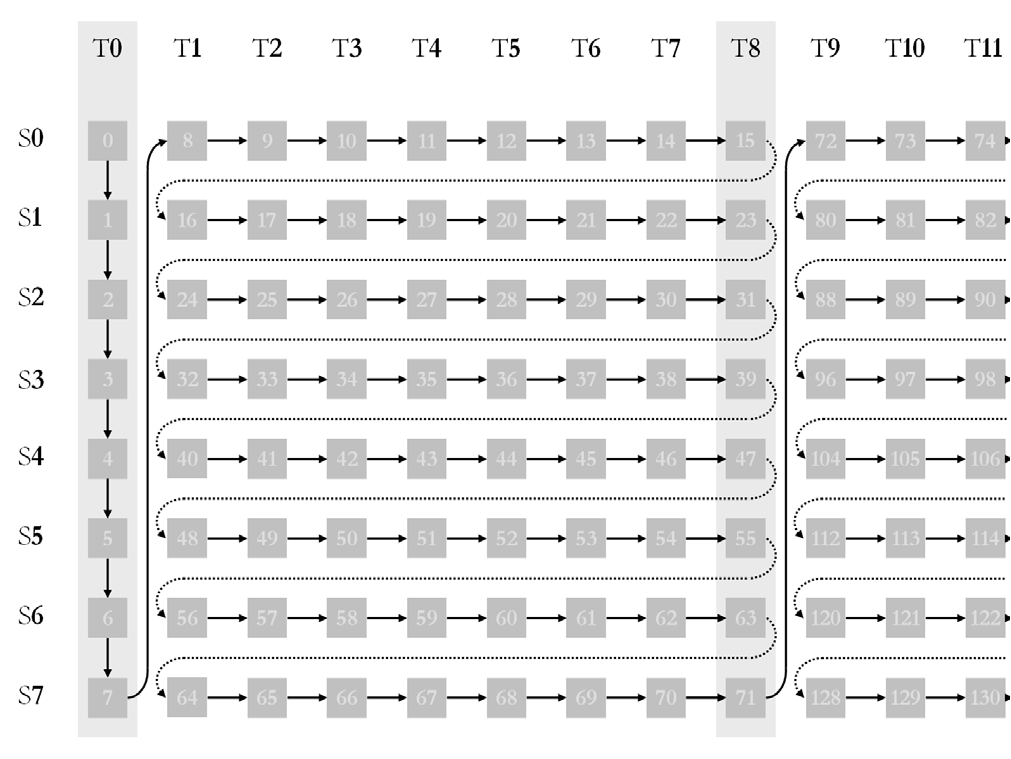
\includegraphics[width=7cm]{../img/encoding-memory}
\end{wrapfigure}

Die beschriebene Kodierungsmethode erlaubt es zudem eine effiziente Anordnung von Rahmen im Datenstrom.\cite{paper}
\texttt{T*} beschreibt hierbei den Zeitpunkt des Rahmens und \texttt{S*} die Perspektive.
Ein signifikanter Vorteil ist hier die Parallelisierung des Dekodierens.
Vor dem Zeitpunkt \texttt{T9} sind alle vorhergehenden Ansichten im Speicher geladen.
Die Ansichten h\"angen jeweils voneinander ab, aber es gibt hierbei immer Paare von ''Quellansichten'' und
''Senkenansichten''.
Die Quellansichten k\"onnen unabh\"angig voneinander dekodiert werden.

\noindent\\ Die Kodierungseffizienz ist hierbei stark abh\"angig von der Videosequenz.\cite{paper}
Im folgenden Diagramm sieht man einen Vergleich von \textit{Peak Signal to Noise Ratios} zwischen \textit{Simulcast}
und der \texttt{MVC}-Implementierung.
Die Variationen sind kein Mangel des Kodierungsverfahrens -welches im Schnitt immer noch eine Verbesserung gegen\"uber
Simulcast ist- vielmehr sind manche Videosequenzen schlichtweg nicht geeignet um per MVC kodiert zu werden.

\begin{center}
    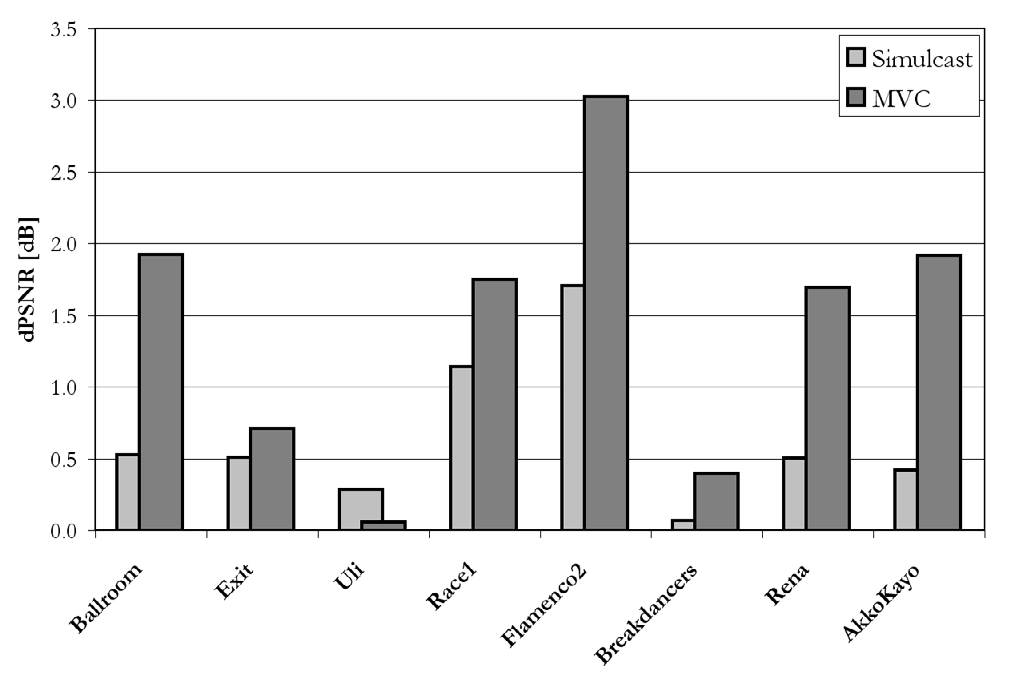
\includegraphics[width=0.75\textwidth]{../img/encoding-efficiency}
\end{center}
\noindent Ein triviales Beispiel hierf\"ur ware eine Sequenz, in welcher zwei 10 cm entfernte Kameras auf ein Objekt
gerichtet sind.
Eine davon ist allerdings auf einen Laternenpfahl gerichtet, an welchem die andere vorbeischaut.
Hierbei g\"abe es offensichtlich au{\ss}er der Lichtatmosph\"are des Bildes kaum Redundanzen.
